% rubber: set program xelatex
\documentclass[10pt, compress, titleprogressbar, aspectratio=169]{beamer}

\usepackage{todo}
\usepackage{marvosym}

\usepackage{pifont,xcolor}% http://ctan.org/pkg/{pifont,xcolor}

\title{\centering{}Bebida Improvements and Optimizations}

\subtitle{REGALE Project WP2}
\date{2023}
\author[Michael Mercier]{%
    \textbf{Michael Mercier - Ryax Technologies}
    }
    \institute[Ryax, REGALE]{%
        %Univ. Grenoble Alpes, Inria, CNRS, \\Grenoble INP, LIG, F-38000 Grenoble, France
        %Bull, Atos technologies\\
        %\includegraphics[width=0.2\paperwidth]{./img/logo_UGA.png}
        %\hspace{.18\textwidth}
        %\includegraphics[width=0.2\paperwidth]{./img/logo_inria.png}}

        
\includegraphics[width=0.2\paperwidth]{./img/logo_RYAX.png}
        
\includegraphics[width=0.2\paperwidth]{./img/logo_REGALE.png}\inst{2}
        \hspace{.55\textwidth}\inst{1}}

        \begin{document}

        \maketitle

        %%%%%%%%%% Bebida %%%%%%%%%%%
        \section{HPC and Big Data Collocation: BeBiDa}

        %\subsection{Resource management convergence}

        \begin{frame}{Resources and Jobs Management System (\textbf{RJMS})}{a.k.a.
            Batch scheduler}
            \begin{columns}
                \begin{column}{0.6\textwidth}
                    \begin{itemize}
                        \item Shares resources between users
                        \item Resources are CPU, Memory, Network bandwidth, \ldots
                        \item Conflicting objectives:
                            \begin{itemize}
                                \item Minimize waiting time
                                \item Maximize jobs throughput
                                \item Maximize cluster utilization
                            \end{itemize}
                        \item Examples:
                            \begin{itemize}
                                \item HPC: SLURM, OAR, PBS, \dots
                                \item Big Data: Hadoop YARN, Kubernetes \dots
                            \end{itemize}
                    \end{itemize}
                    \begin{center}
                        
\includegraphics[width=0.15\linewidth,height=\textheight,keepaspectratio]{./img/oar_logo.png}
                        \hspace{0.3cm}
                        
\includegraphics[width=0.15\linewidth,height=\textheight,keepaspectratio]{./img/slurm_logo.png}
                        \hspace{0.3cm}
                        
\includegraphics[width=0.15\linewidth,height=\textheight,keepaspectratio]{./img/hadoop_logo.jpg}
                        \hspace{0.3cm}
                        
\includegraphics[width=0.15\linewidth,height=\textheight,keepaspectratio]{./img/k8s_logo.png}
                    \end{center}
                    \vfill
                    \hspace{2em}
                    \textbf{RJMS are complex: \\
                    \hspace{2em}
                    SLURM and YARN $\simeq$ 400k lines of code}
                    \vfill
                \end{column}
                \begin{column}{0.4\textwidth}
                    \begin{center}
                        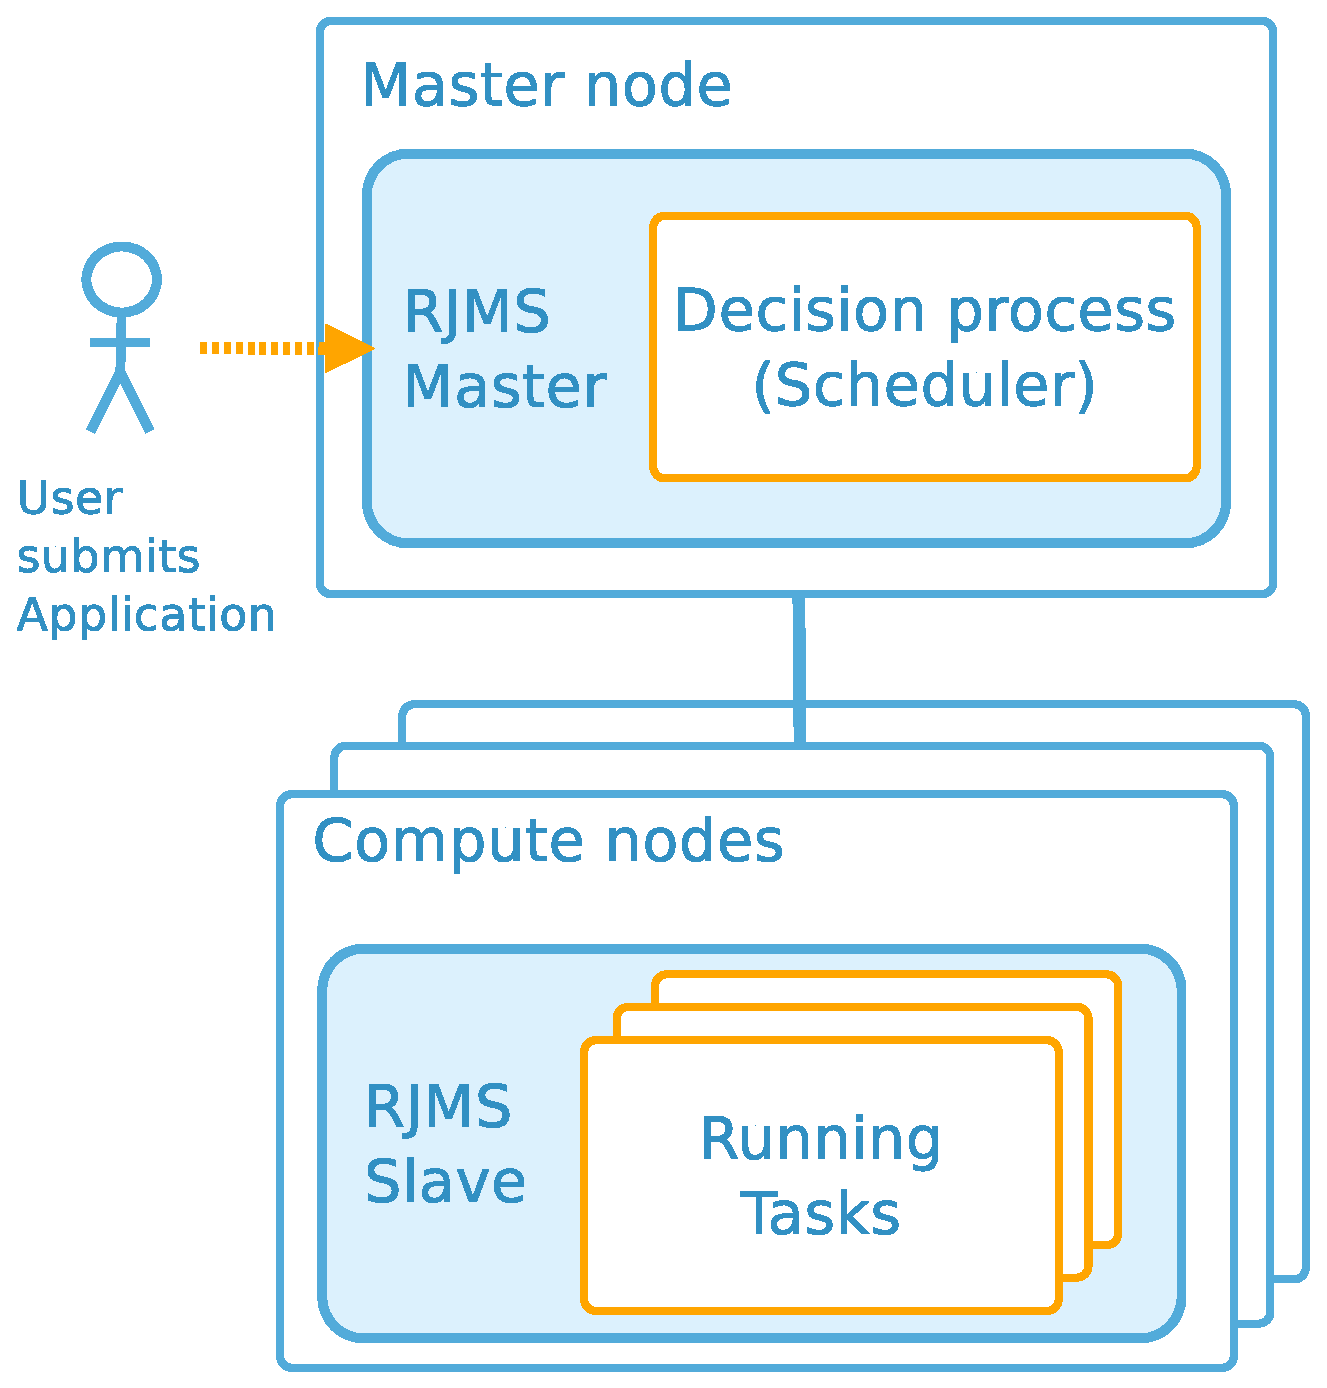
\includegraphics[width=\linewidth,height=\textheight,keepaspectratio]{./img/rjms_overview.eps}
                    \end{center}
                \end{column}
            \end{columns}
        \end{frame}

        \begin{frame}{What's happening today}{Static partitioning}
            \begin{columns}
                \begin{column}{0.7\textwidth}
                    \begin{center}
                        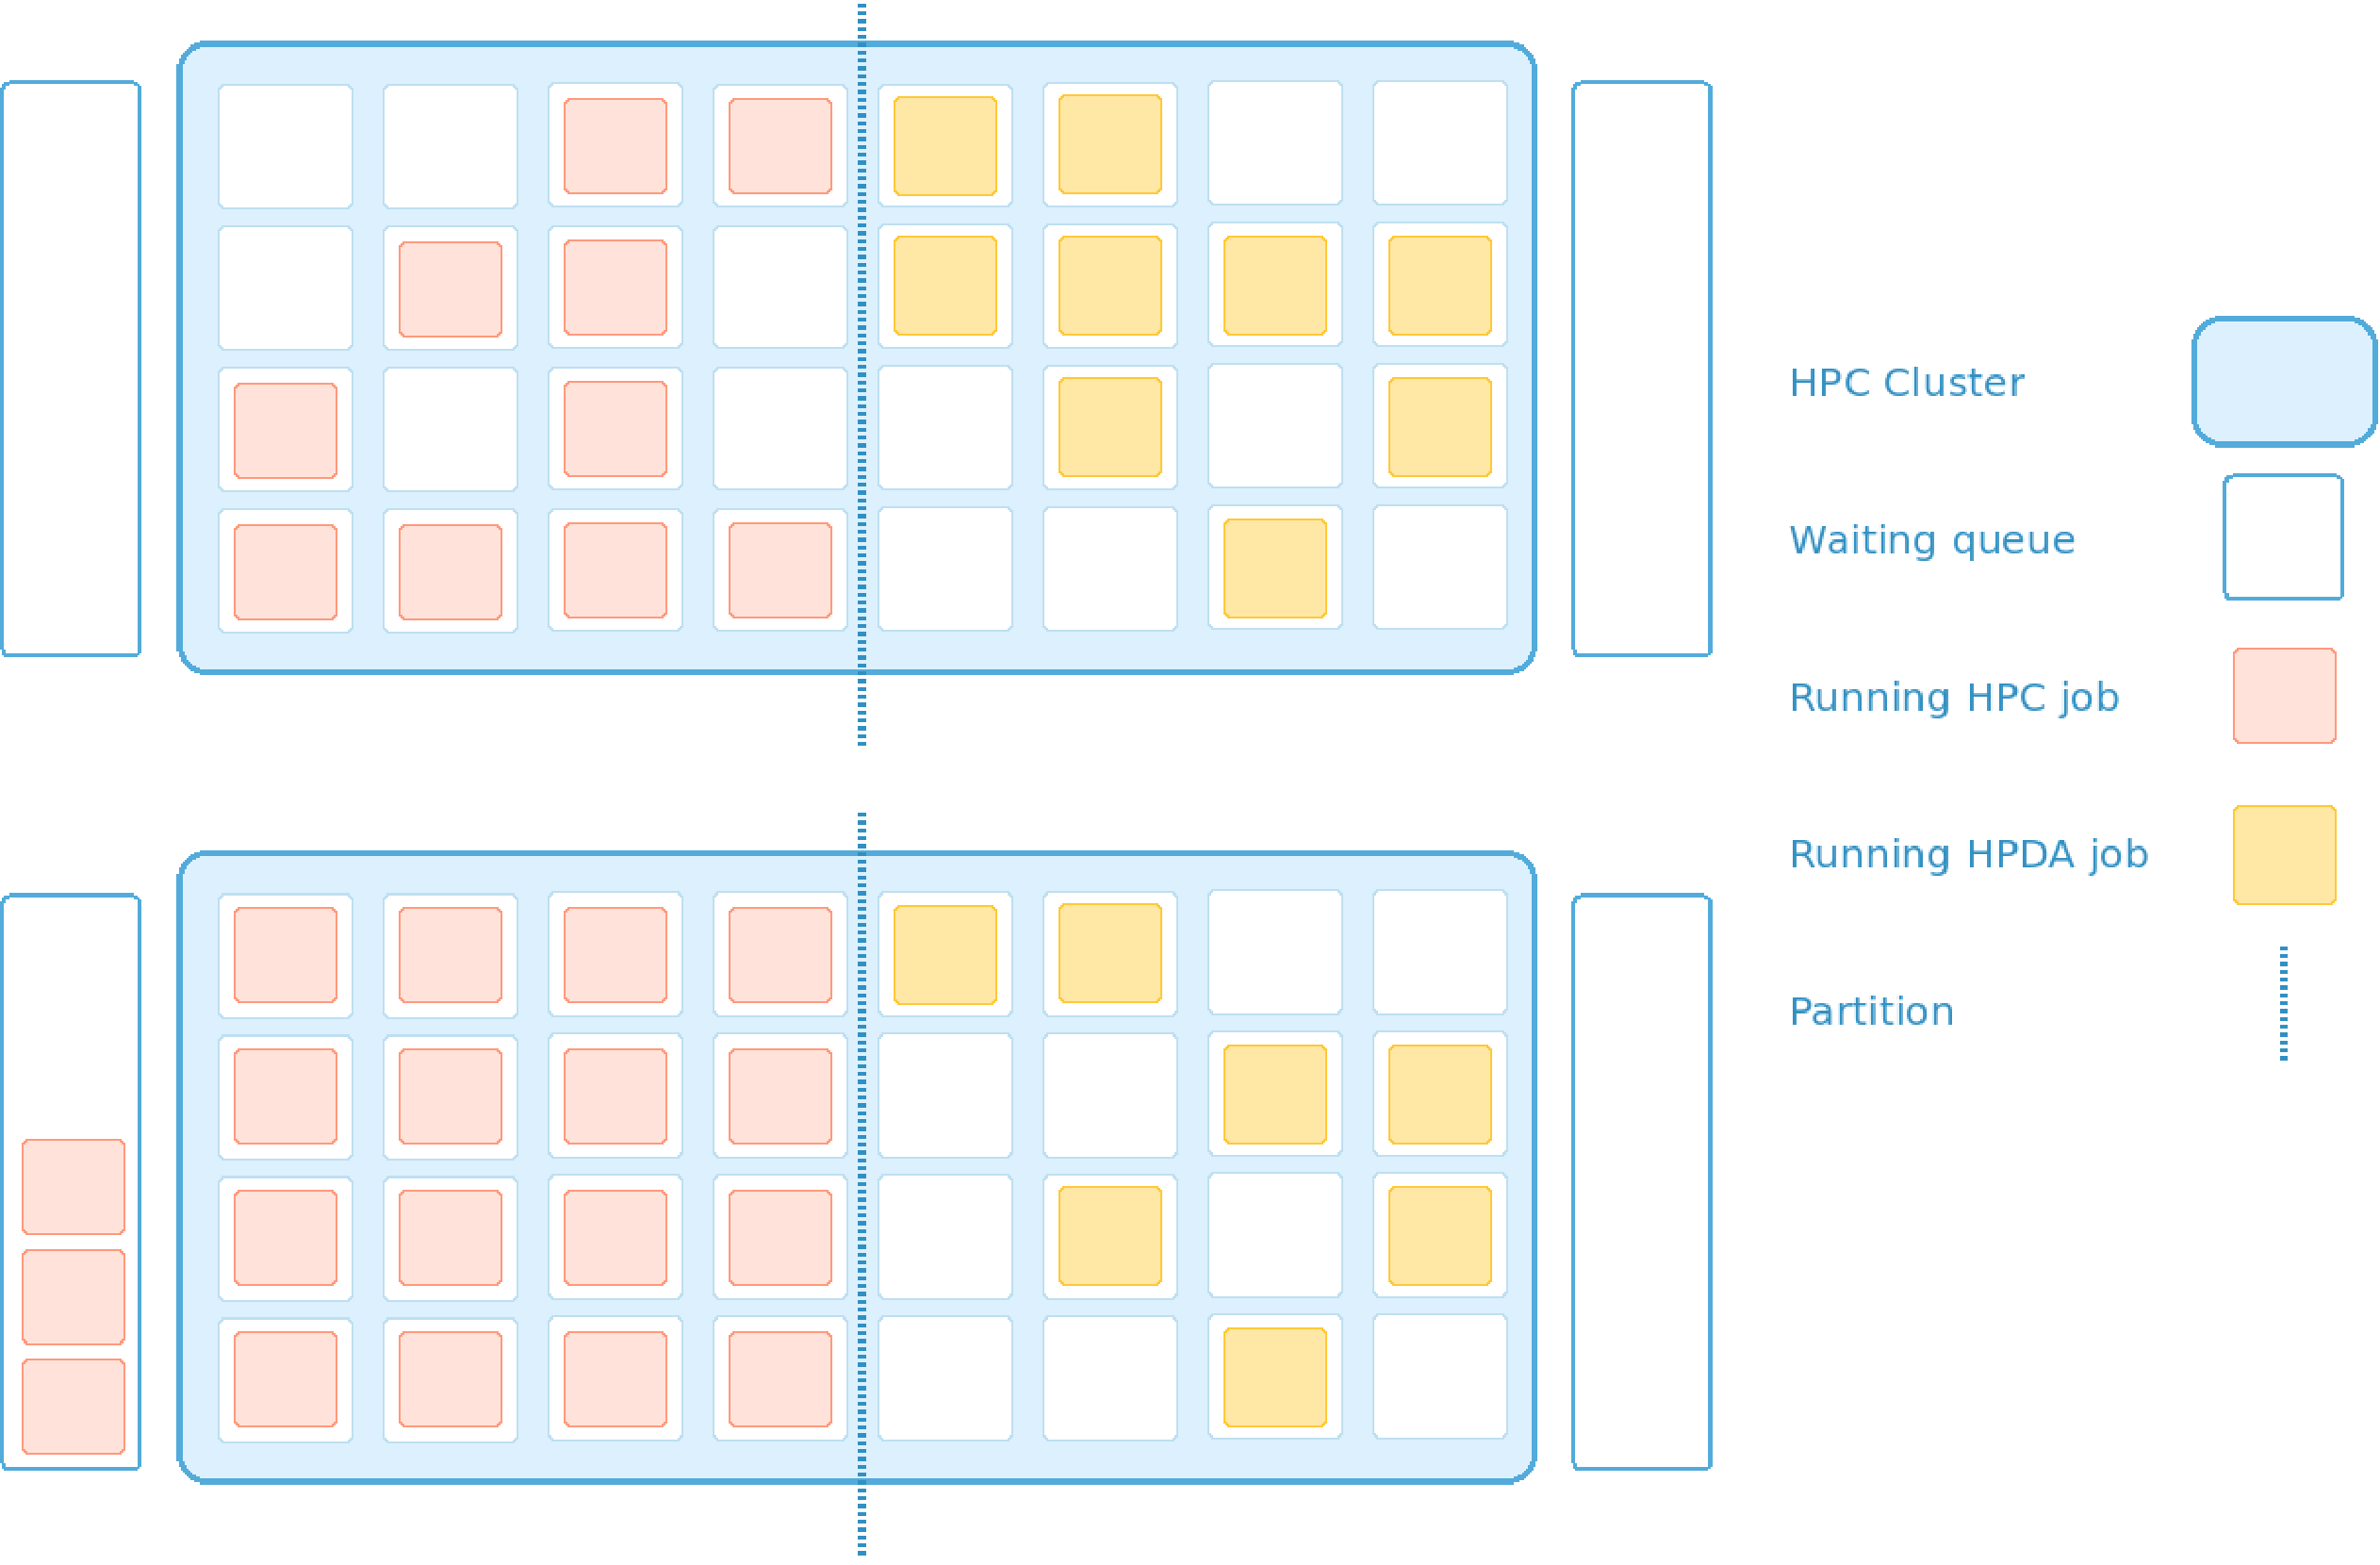
\includegraphics[width=\linewidth,height=\textheight,keepaspectratio]{./img/static_partition}
                    \end{center}
                \end{column}
                \begin{column}{0.3\textwidth}
                    \textbf{Static cluster partitioning:}
                    \begin{itemize}
                        \item Simple workload discrimination
                        \item No node sharing
                    \end{itemize}
                    \vspace{2em}

                    \textbf{Leads to resources waste!}
                    \begin{itemize}
                        \item When one queue is filling up
                        \item Available nodes on the other partition are not used
                    \end{itemize}
                \end{column}
            \end{columns}

        \end{frame}

        \begin{frame}{What we want to achieve}{Dynamic sharing}
            %\begin{columns}
            %    \begin{column}{0.3\textwidth}
            %        \begin{itemize}
            %            \item Dynamic resource allocation
            %                \vspace{1em}
            %            \item Full cluster utilization
            %                \vspace{1em}
            %            \item Co-scheduling (if it make sense)
            %        \end{itemize}
            %    \end{column}
            %    \begin{column}{0.7\textwidth}
            \begin{center}
                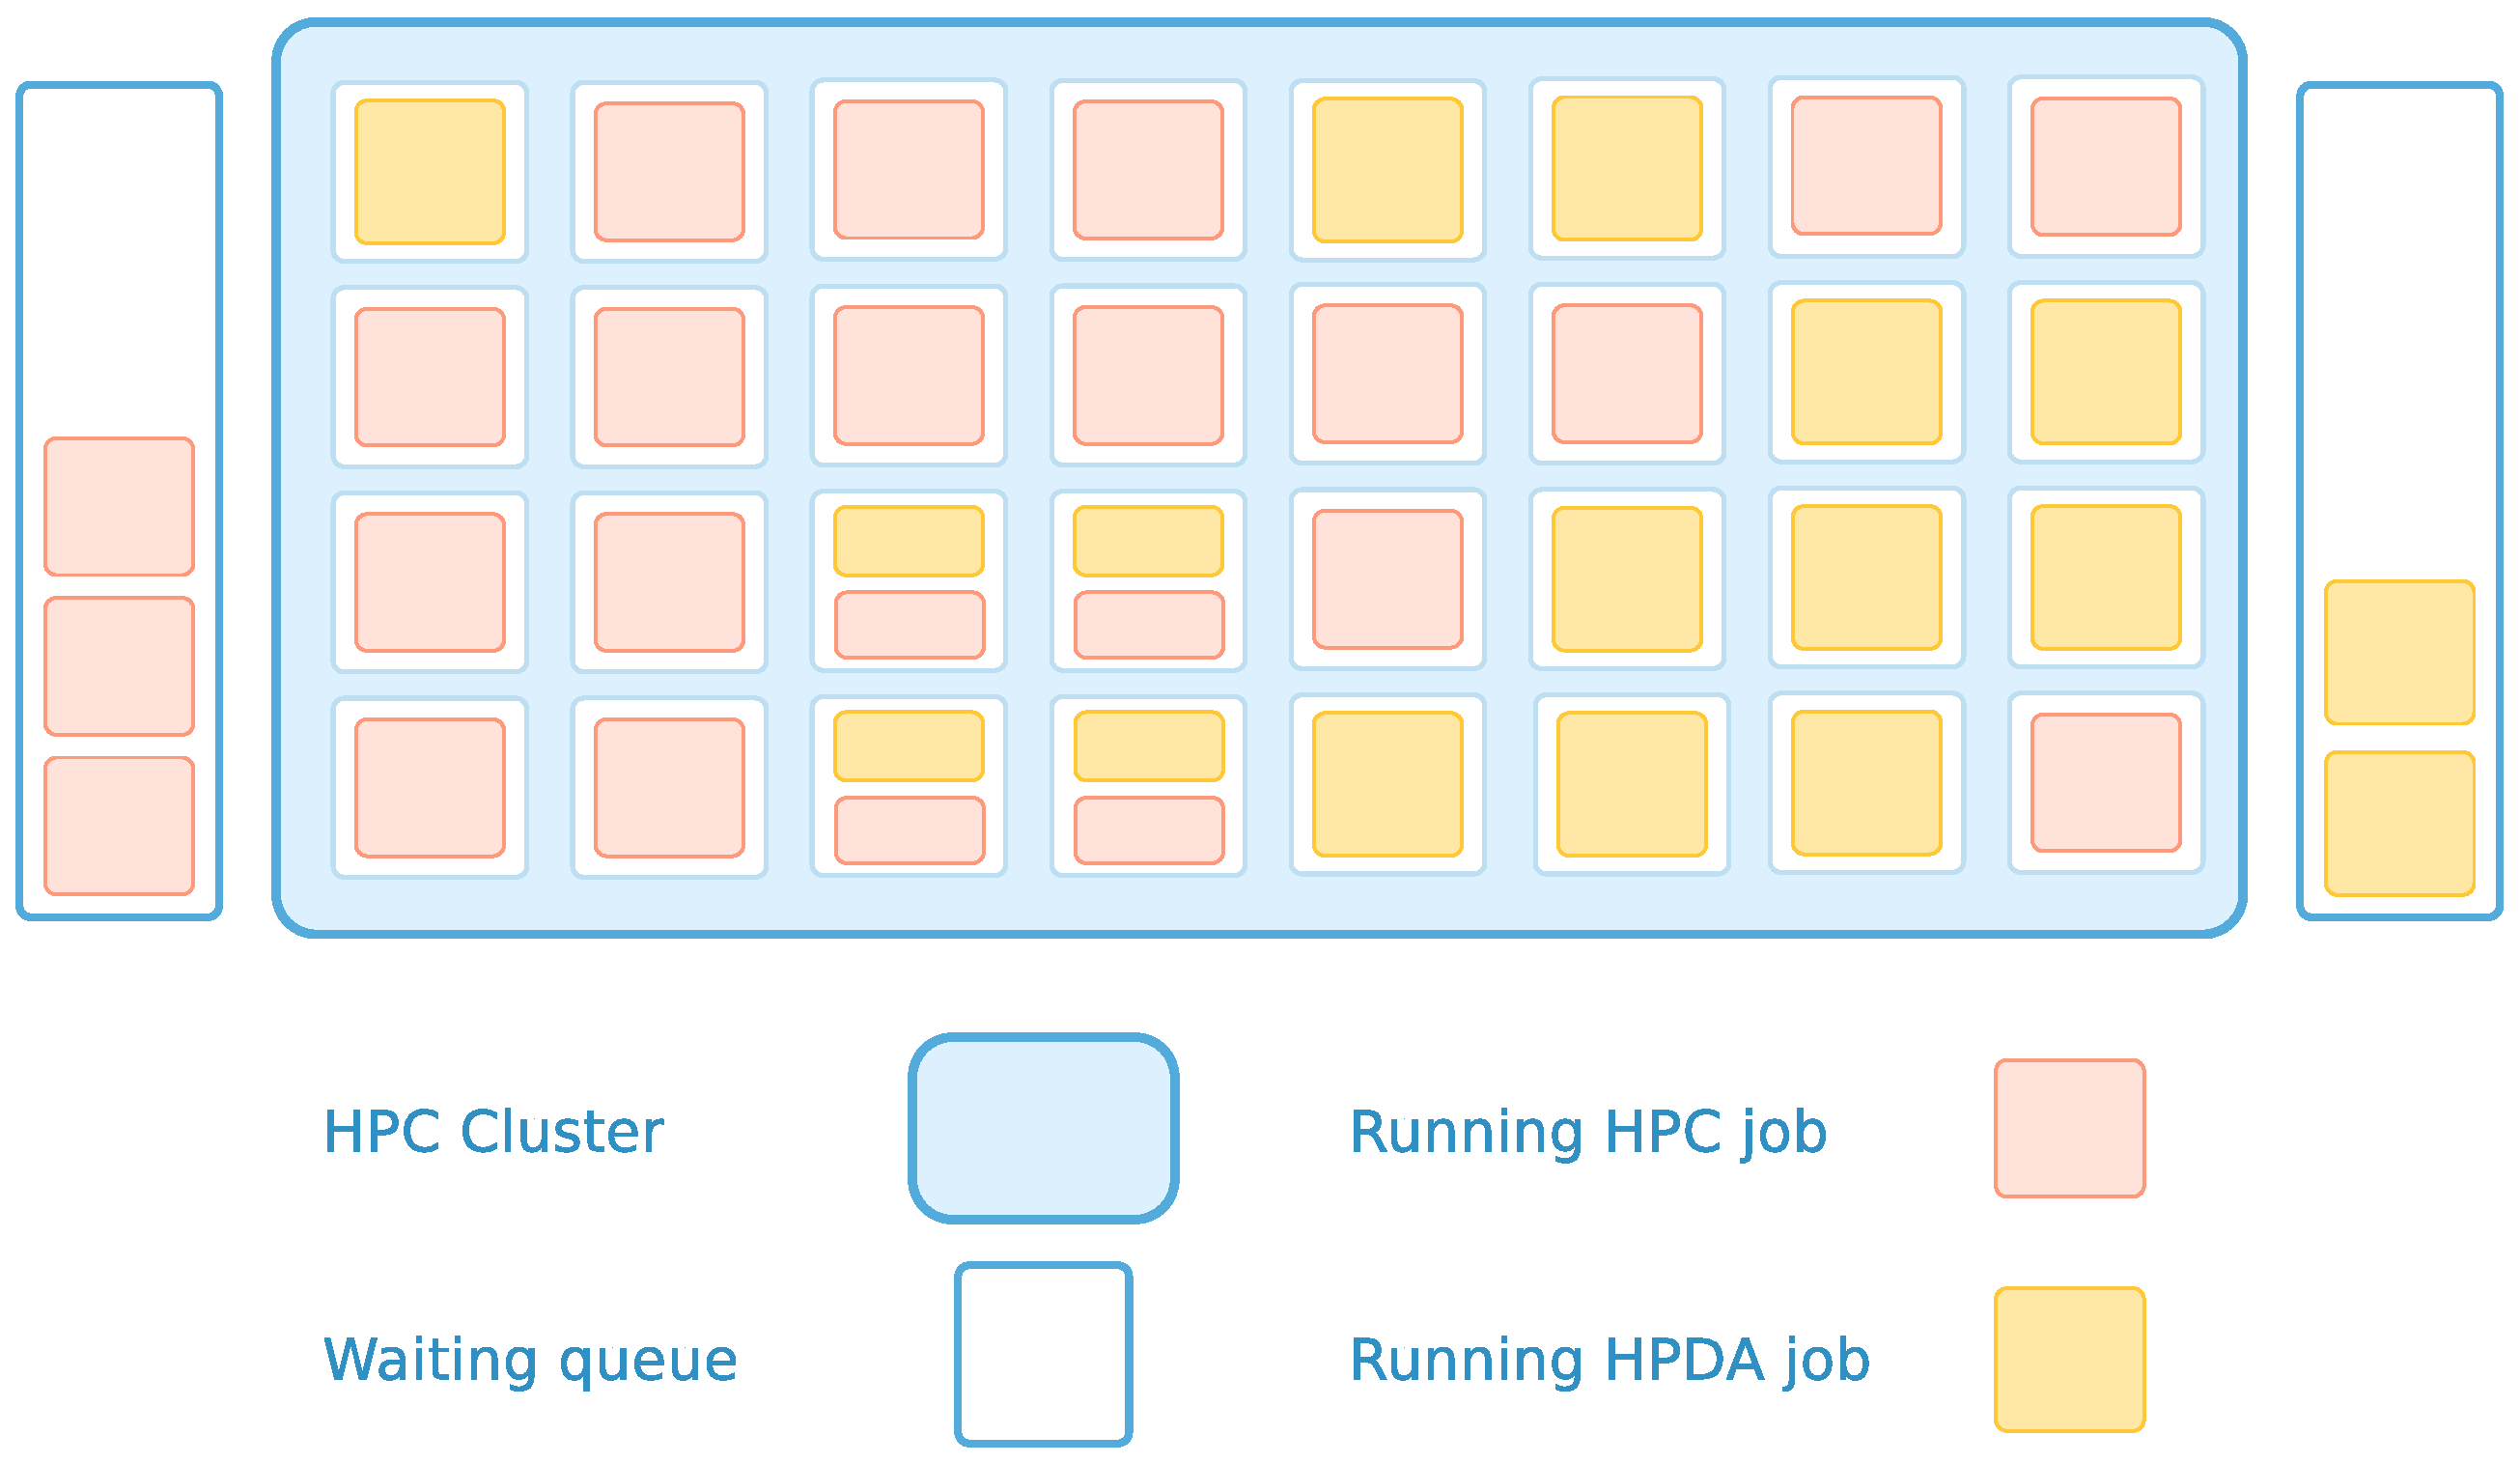
\includegraphics[width=\linewidth,height=\textheight,keepaspectratio]{./img/mixed_workload_cluster.eps}
            \end{center}
            %    \end{column}
            %\end{columns}
        \end{frame}

        \begin{frame}{An analogy}{Is the Jar Full?}
            \vspace{1mm}
            %  \begin{columns}
            %    \begin{column}{0.5\textwidth}
            \centering
            
\includegraphics[width=\linewidth,height=\textheight,keepaspectratio]{./img/stones.jpg}
            %    \end{column}
            %    \begin{column}{0.5\textwidth}
            %      \centering
            %      \includegraphics[width=\linewidth,height=\textheight,keepaspectratio]{./img/sand.jpg}
            %    \end{column}
            %  \end{columns}
        \end{frame}

        \begin{frame}{A Scheduling Problem}{Solutions}
            \vspace{1mm}
            \centering
            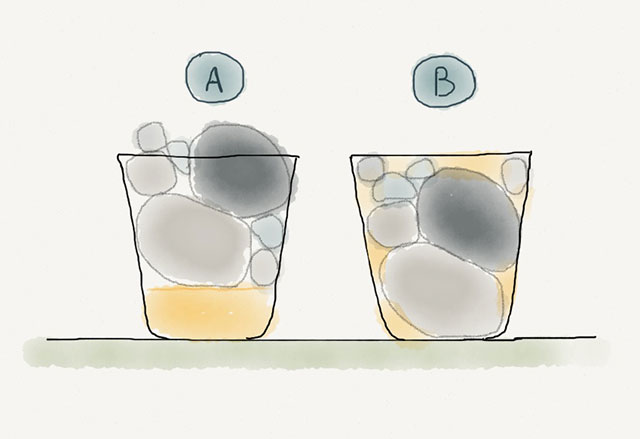
\includegraphics[width=\linewidth,height=\textheight,keepaspectratio]{./img/stones_and_sand.jpg}
        \end{frame}

        \begin{frame}{Big Data and HPC workload Collocation}{At the Resource Management Level}
            \begin{columns}
                \begin{column}[c]{0.4\textwidth}
                    \textbf{Jar: HPC Hardware Cluster}
                    \begin{itemize}
                        \item Resources (CPU cores)
                        \item Time (seconds)
                    \end{itemize}
                    \textbf{Stones: HPC Jobs}
                    \begin{itemize}
                        \item Static resource allocation
                        \item Static time allocation
                    \end{itemize}
                    \pause
                    \begin{block}{\textbf{Sand: Big Data Applications}}
                        \begin{itemize}
                            \item Dynamic resource allocation
                            \item Resilient to resource preemption
                        \end{itemize}
                    \end{block}
                \end{column}
                \begin{column}{0.6\textwidth}
                    \begin{center}
                        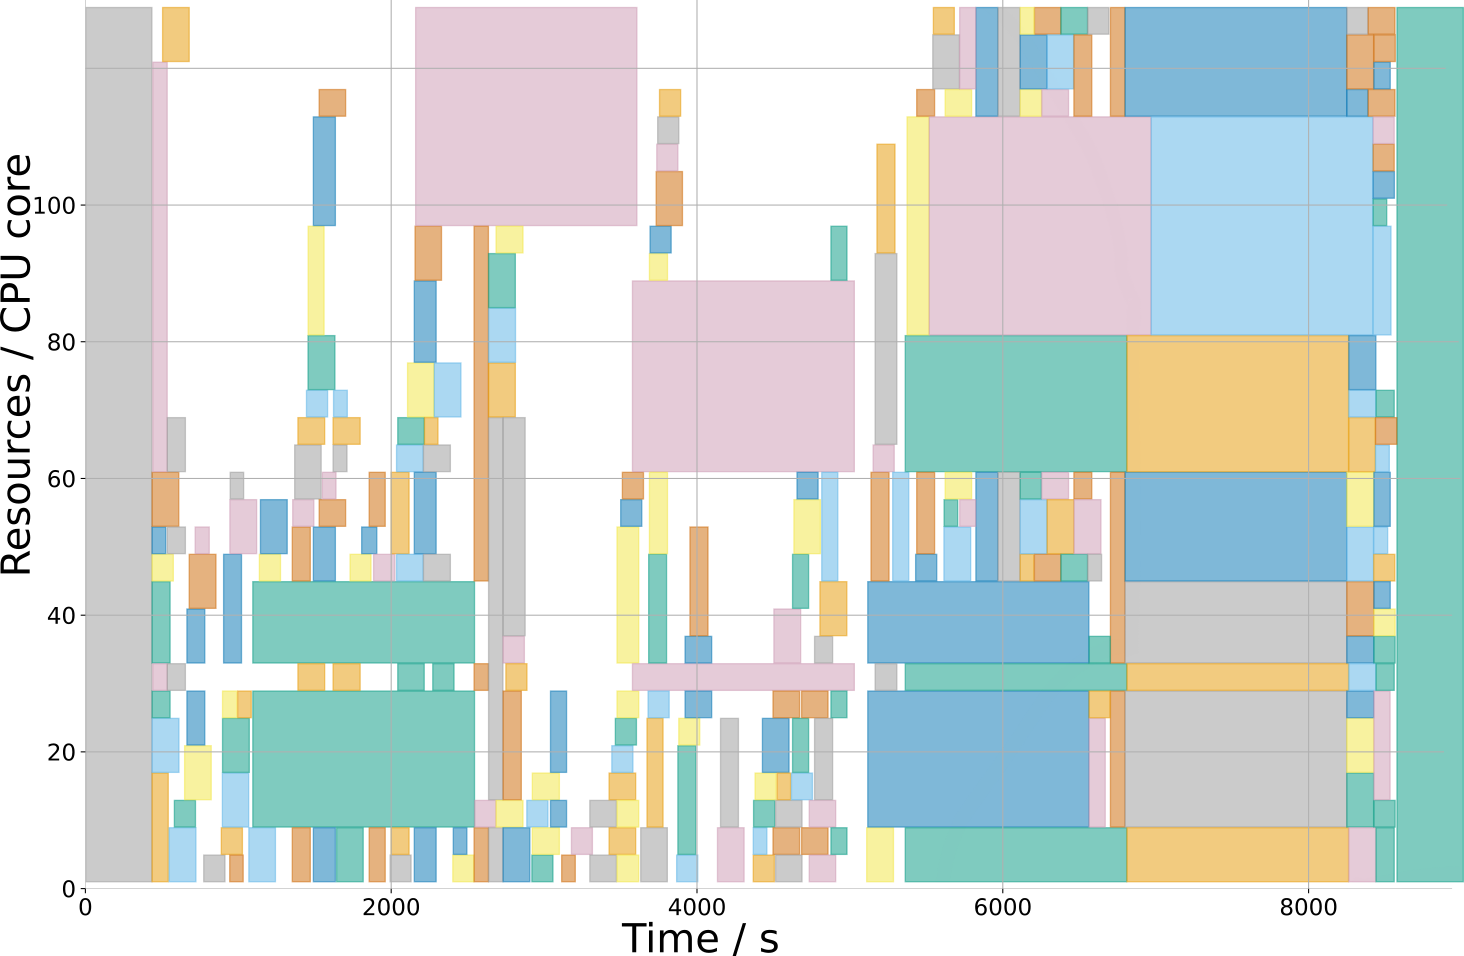
\includegraphics[width=\linewidth,height=\textheight,keepaspectratio]{./img/gantt_small.png}
                    \end{center}
                \end{column}
            \end{columns}
        \end{frame}

        \begin{frame}{Existing Approaches for Collocation}{Related Works}
            \begin{columns}
                \begin{column}[t]{0.45\textwidth}
                    \textbf{BigData in HPC job}
                    \begin{itemize}
                        \item Setup/teardown at every job
                        \item Need to import/export data
                    \end{itemize}
                    \vspace{0.5em}
                    \textbf{Two-level Scheduling}
                    \begin{itemize}
                        \item Dynamically resources sharing negotiation
                        \item Increase operational cost
                        \item New API implementation required
                    \end{itemize}
                    \textbf{Examples:} Mesos, Omega, Grid Engine\\
                    \vspace{0.5em}
                    \textbf{The major problem is complexity:\\=> from 5k to 50k lines of code}
                    \vspace{0.5em}
                    %\\\small\texttt{More detailed comparison in the thesis.}
                \end{column}
                \begin{column}[t]{0.5\textwidth}
                    \textbf{RJMS adaptor}
                    \begin{itemize}
                        \item HPC RJMS provides resources to Big Data
                        \item Convert BigData resource requests
                            %\item Coupling the two management system
                        \item Walltime problem
                    \end{itemize}
                    \textbf{Examples:} Neves et al. (Euro-Par 2012),\\\hspace{2em}Intel YARN adaptor
                    \begin{center}
                        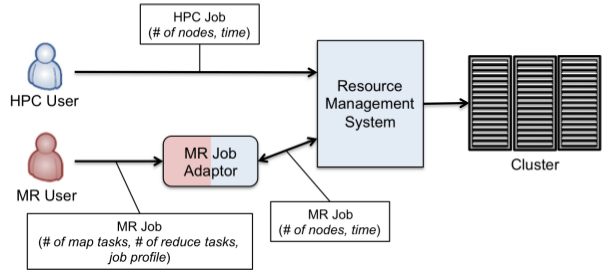
\includegraphics[width=0.8\linewidth,height=\textheight,keepaspectratio]{./img/scheduler_adaptor.png}
                    \end{center}
                \end{column}
            \end{columns}
        \end{frame}


        \begin{frame}{Keep it Simple}{Requirements}
            \begin{center}
                \begin{minipage}{0.70\textwidth}
                    \begin{exampleblock}{We wants our solution to:}
                        \begin{enumerate}
                            \item \textbf{Use existing tools unmodified} (RJMS + Applications)
                                \vspace{1em}
                            \item \textbf{Work for any RJMS}
                                \vspace{1em}
                            \item \textbf{Transparent for users}
                                \vspace{1em}
                            \item \textbf{Minimal disturbance to HPC jobs} from Big Data applications
                                \vspace{1em}
                            \item \textbf{Leverage Big Data dynamicity and resilience}
                        \end{enumerate}
                    \end{exampleblock}
                \end{minipage}
            \end{center}
        \end{frame}

        \begin{frame}{BeBiDa: Best effort Big Data on HPC cluster}{%
                Using HPC idle resources for Big Data analytics}
                \begin{columns}
                    \begin{column}{0.40\textwidth}
                        \textbf{HPC: job's prolog/epilog (50 LoC)\\
                        \vspace{1em}
                        BigData: resources \{de\}commission}
                        \vspace{1em}
                        \begin{enumerate}
                            \item \textit{Initially:}\\Nodes are attached to the Big Data resource pool
                                \vspace{1em}
                            \item \textit{When an HPC job starts:}\\Prologue decommissions the resources
                                \vspace{1em}
                            \item \textit{When an HPC job finishes:}\\Epilogue is giving resources back
                        \end{enumerate}
                    \end{column}
                    \begin{column}{0.60\textwidth}
                        \begin{center}
                            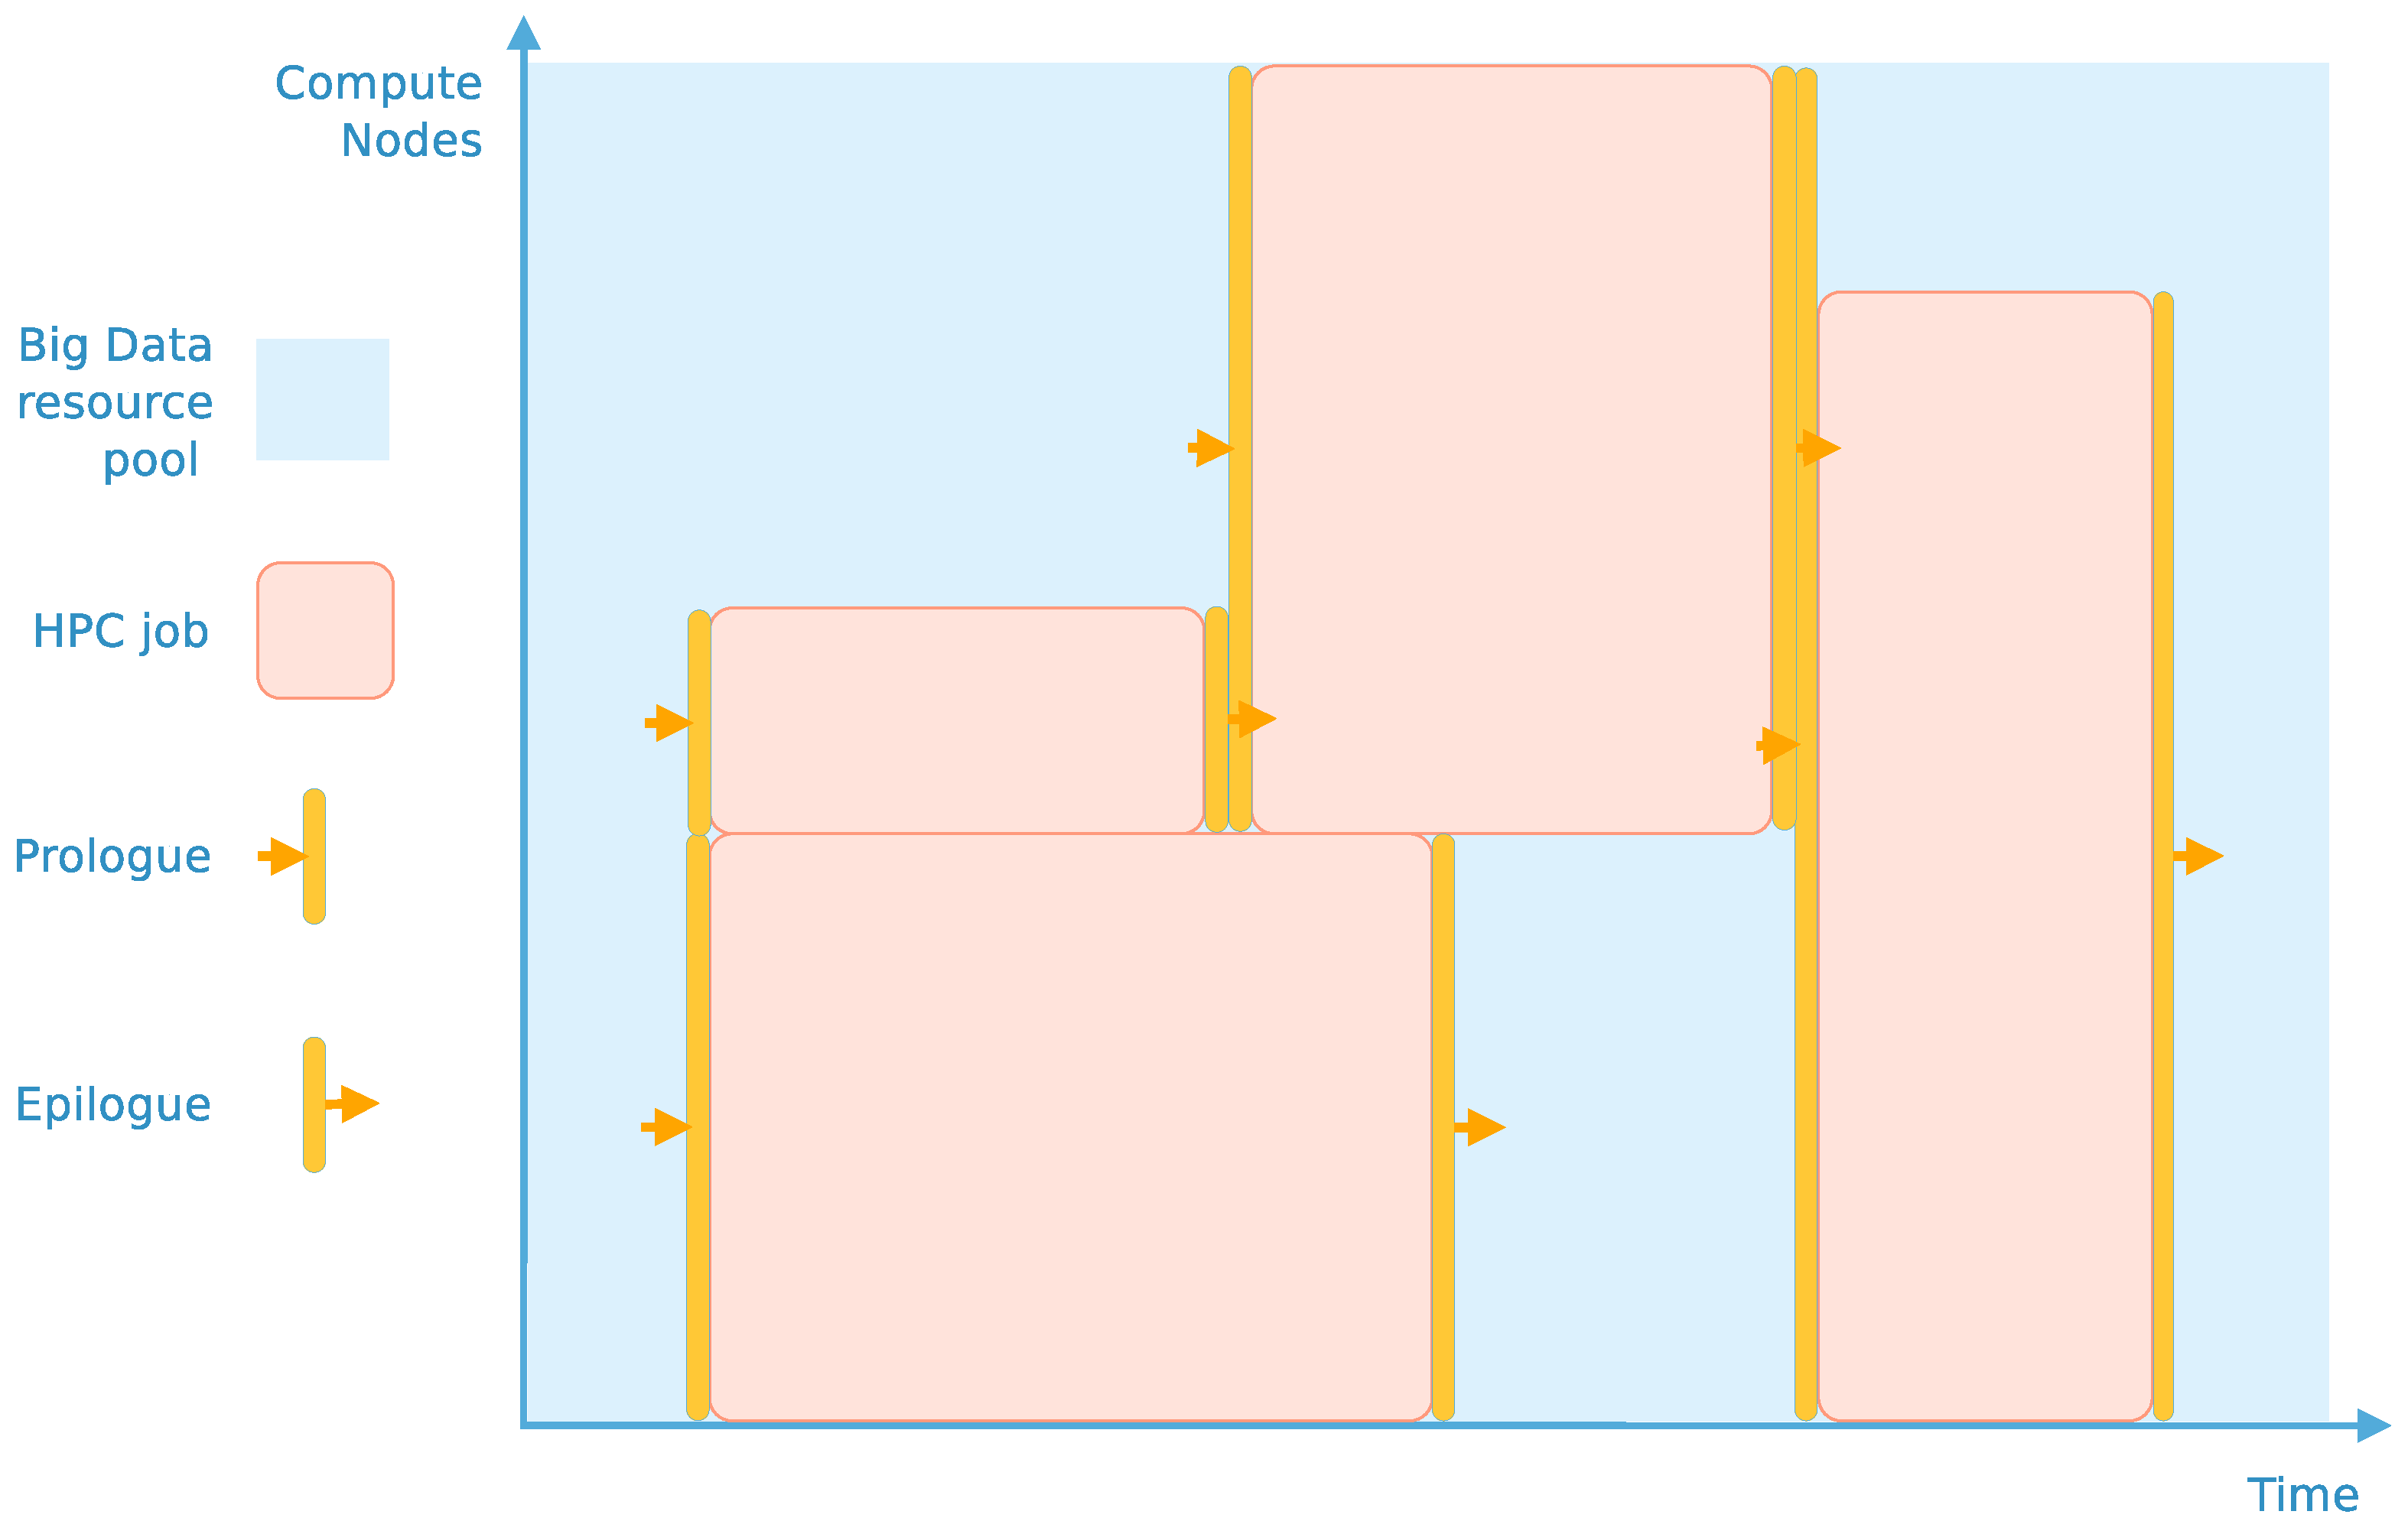
\includegraphics[width=\linewidth,height=\textheight,keepaspectratio]{./img/BeBiDa_gantt_blind.eps}
                        \end{center}
                    \end{column}
                \end{columns}
        \end{frame}

        \begin{frame}{BeBida Working Example}{From 70\% to 100\% utilization}
            \begin{center}
                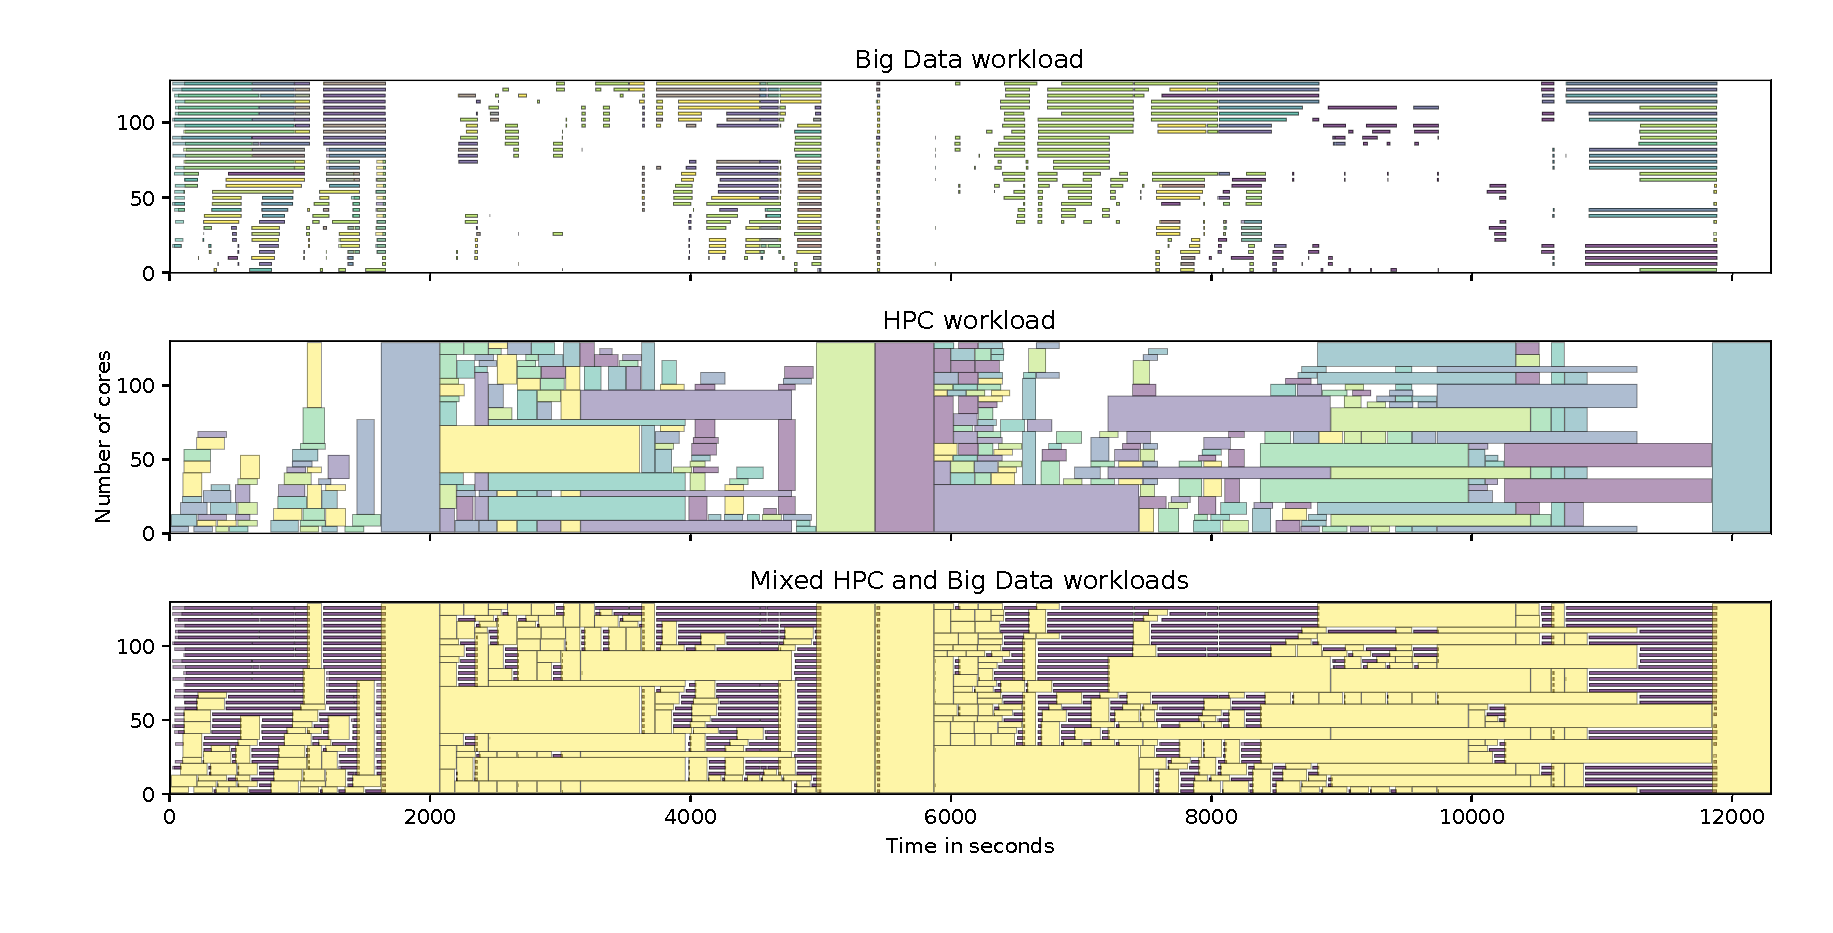
\includegraphics[width=\linewidth, height=\textheight, keepaspectratio]{./img/fig/gantt_example}
            \end{center}
        \end{frame}


        \begin{frame}{Resource Preemption Impact on Big Data}{Measure effective computation time}
            \begin{columns}
                \begin{column}{0.4\textwidth}
                    \begin{block}{Time Effectiveness}
                        % TODO make it more simple
                        %Effective computation time over\\Total computation time
                        $$E = \frac{Useful\ computation\ time}{Total\ computation\ time}$$
                        %$$E = \frac{\sum{T_{completed}} - \sum{T_{recomputed}}}{\sum{T_{completed}} + \sum{T_{aborted}}}$$
                    \end{block}

                    Variability root causes:
                    \begin{itemize}
                        \item HPC workloads shape
                        \item Big Data workload applications sensitivity
                        \item Coincidence between "holes" and large applications
                        \item System noise
                    \end{itemize}
                \end{column}
                \begin{column}{0.6\textwidth}
                    \begin{center}
                        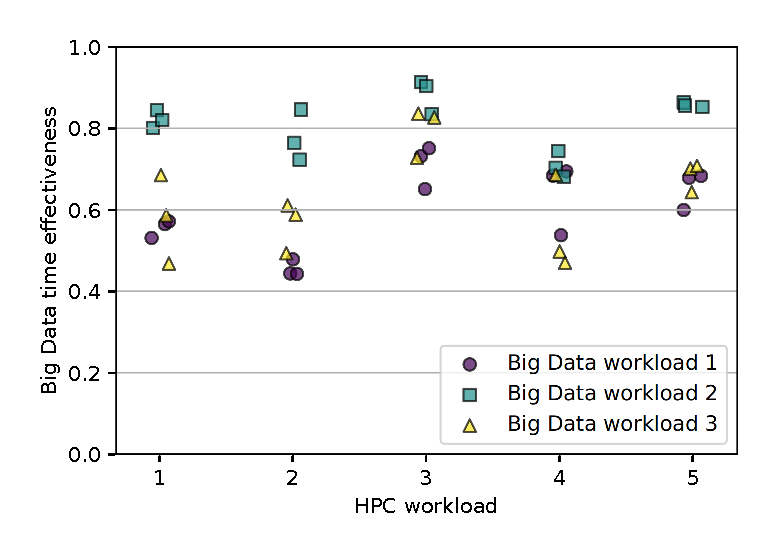
\includegraphics[width=\linewidth, height=\textheight, keepaspectratio]{./img/fig/Big_data_effectiveness_sum}
                    \end{center}
                \end{column}
            \end{columns}
        \end{frame}

        \begin{frame}{Overhead on HPC Workloads}{With and without BeBiDa}
            \begin{columns}
                \begin{column}{0.38\textwidth}
                    \begin{block}{Mean Execution Time}
                        +6\% on average with BeBiDa
                    \end{block}
                    \begin{exampleblock}{Mean Waiting Time}
                        \begin{itemize}
                            \item epilog/prolog: < 16s\\
                            \item 26\% (1min) to 1\% (30min) of the jobs execution time
                            \item +17\% on average with BeBiDa
                        \end{itemize}
                    \end{exampleblock}
                    Variability root causes:
                    \begin{itemize}
                        \item Scheduling anomalies
                        \item Network contentions
                        \item DFS daemon
                    \end{itemize}

                \end{column}
                \begin{column}{0.58\textwidth}
                    \begin{center}
                        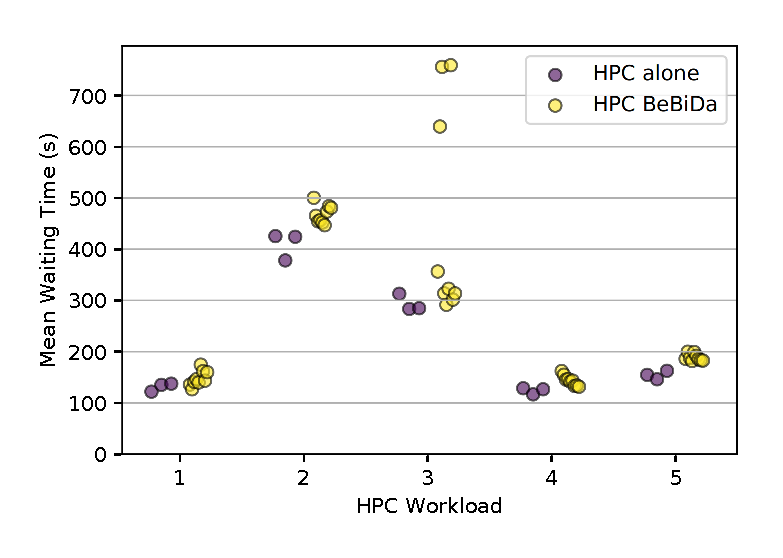
\includegraphics[width=\linewidth, height=\textheight, keepaspectratio]{./img/fig/HPC_metrics.eps}
                    \end{center}
                \end{column}
            \end{columns}
        \end{frame}

        \begin{frame}{Key Characteristics}{Advantages and Drawbacks}
            \begin{columns}
                \begin{column}{0.4\textwidth}
                    \begin{alertblock}{Performance impact}
                        \begin{itemize}
                            \item HPC execution time +6\% on average
                            \item HPC waiting time +17\% on average
                            \item High variability in Big Data efficiency (68\% on average)
                        \end{itemize}
                    \end{alertblock}

                \end{column}
                \begin{column}{0.55\textwidth}
                    \begin{exampleblock}{BeBiDa main advantages}
                        \begin{itemize}
                            \item Use any existing RJMSs without modification
                            \item Transparent for users
                            \item HPC workload has priority
                            \item Only $\simeq$ 50 lines of code + configuration\\
                                \vspace{0.5em}
                                \textbf{100 to 1000 times less code}
                            \item Increase the cluster utilization
                            \item Uses resources that would be idle otherwise
                        \end{itemize}
                    \end{exampleblock}
                \end{column}
            \end{columns}
            \vspace{1em}
            \large\textbf{Fully reproducible experiments and analysis:}\\
            \url{https://gitlab.inria.fr/mmercier/bebida/}
        \end{frame}

        \section{Bebida Optimizations}

        \begin{frame}{REGALE Use cases}{and Optimizations}
            \begin{columns}
                \begin{column}{0.45\textwidth}
            \begin{exampleblock}{Spark Application for:}
                \begin{enumerate}
                    \item Hydrological flow analysis (Pilot 4)
                    \item Network security analysis (Pilot 3)
                \end{enumerate}
            \end{exampleblock}
            \hfill \break
            We want more guarantees:
            \begin{itemize}
                \item \textbf{Deadline aware} (1):\\ Run before a user-defined deadline
                \item \textbf{Time critical} (2):\\ Run as fast as possible
            \end{itemize}
                \end{column}
                \begin{column}{0.55\textwidth}
                    \begin{center}
                        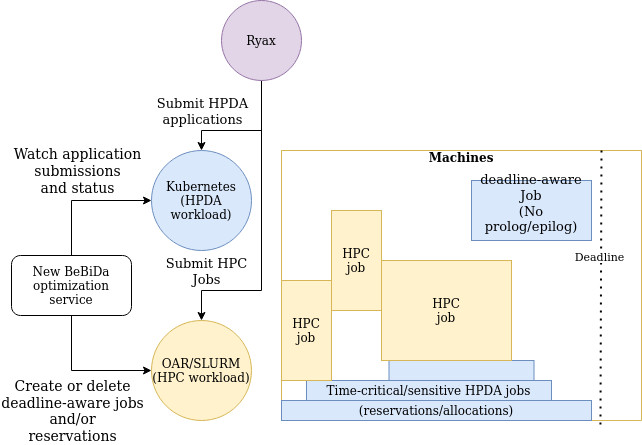
\includegraphics[width=\linewidth, height=\textheight, keepaspectratio]{../figureBOS.png}
                    \end{center}
                \end{column}
            \end{columns}
        \end{frame}

        \begin{frame}{Bebida Optimization Service}{Roadmap}
            \begin{itemize}
                \item[$\boxtimes$]
                    First implementation with simple heuristic (Ti'Punch):\\
                    based on threshold on the number of pending job in the BDA queue, create HPC
                    jobs that will stay in the BDA resource pool.
                \item[$\boxtimes$]
                    support for K8s (BDA)
                \item[$\boxtimes$]
                    support Slurm over SSH (HPC)
                \item[$\boxtimes$]
                    Full testing environment
                \item[$\boxtimes$]
                    Handle BDA app early termination (cancel HPC job if not used anymore)
                \item[$\square$]
                    \textbf{Support for OAR (HPC)}
                \item[$\square$]
                    Handle HPC job termination
                \item[$\square$]
                    Improve heuristic using BDA app time and resource requirements
            \end{itemize}
        \end{frame}

        \begin{frame}{Hackathon Plan}
            \begin{block}{Respond to}
                \begin{itemize}
                    \item
                        Which version of OAR to use?\\
                        =\textgreater{} 2 or 3?
                    \item
                        How to create a container-based testbed for Bebida with OAR and K8s?\\
                        =\textgreater{} NXC or docker compose?
                    \item
                        What is the best way to implement the deadline?\\
                        =\textgreater{} Advanced reservation? Deadline aware jobs?
                    \item
                        What is the best way to implement the time-critical?\\
                        =\textgreater{} Priorities? Co-system? Walltime-less?
                    \item
                        How to connect to OAR?\\
                        =\textgreater{} REST API or SSH + commands?
                \end{itemize}
                \hfill \break
                \centering{}
                \textbf{Let's Hack ! B-)}
            \end{block}
        \end{frame}
    \end{document}
